\subsection{Display driver}
In this section we will describe the hardware and software interface for the display.
Since the display runs best at 3.3 volts we decided to make a small circuit to facilite this, 
even though it says in the datasheet\cite[p. 17]{philips:pcd8544} that it can run on 5 volts.

\subsubsection{PCD8544 - Hardware}
For interfaceing the display we are using a hex buffer that we supply with 3.3V this enables us to run the output from the
microprocessor to the buffer at 5V and then the buffer shifts the level down to 3.3V\cite[p. 1]{STMicroelectronics:HCF4050B}.

To make the 3.3V we are using an LM317L that can take the 5V supply by the STK kit and convert it to 3.3V. 
We made a small circuit that can be seen in 

\improvement{Insert diagram here}

The circuit is quite simple and consist of the LM317 and the HCF4050B hex buffer and two resistors for the LM317.
Since all the buffer does is change the level the inputs to the buffer from the atmega maps to the output of the buffer to the screen.


\subsubsection{PCD8544 - Software}
For the software part of the display there are a couple of things that we need to focus on. 
Firstly there is a clear and easy way to reset the panel to a know state. Efter a reset we need to do some setup for the display to work.
This consists of setting the bias and the voltage to the LCD driver.

\subsubsection{Setup}
First of all we need to issue a reset to the display before we set it up.

\begin{figure}
	\centering
	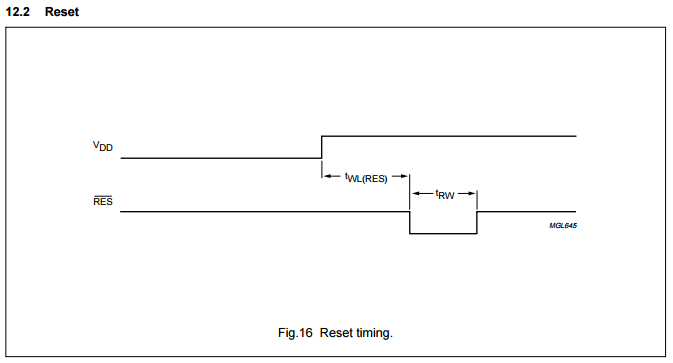
\includegraphics[width=.5\textwidth]{implementation/pcd8544_resetTiming}
	\caption{Reset state for the PCD8544\cite[p. 21]{philips:pcd8544}}
	\label{fig:pcd8544_resetTiming}
\end{figure}

As seen in figure \ref{fig:pcd8544_resetTiming} we need to pull the reset line low to reset the panel.
The timing can be found in til datasheet and it is a minimum of 100ms. that the reset line needs to be low.


The state of the display after a reset can be seen in the datasheet.

\begin{figure}
	\centering
	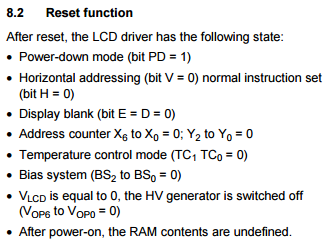
\includegraphics[width=.5\textwidth]{implementation/pcd8544_reset}
	\caption{Reset state for the PCD8544\cite[p. 15]{philips:pcd8544}}
	\label{fig:pcd8544_reset}
\end{figure}

Here we see that we need to do a couple things the get going after the reset we need to set the powermode to active,
we also need to change to the extended instruction set so that we can set the operation voltage.
After this we need to change back to the basic instruction set and then set the display mode in ourcase we want normal.

Since the RAM contents are undefined we should also set these to a know state.
After we have done this we should be ready to use the panel.

The driver implements the proper sequence of commands in its constructor.

\subsubsection{Transferring data/commands}
Since we are using the SPI driver all we need to concern ourselves with is when Transferring data/commands is setting the serialclock enable pin and det data/command pin.
The serialclock and the data out is handeled in the SPI driver.

\begin{figure}
	\centering
	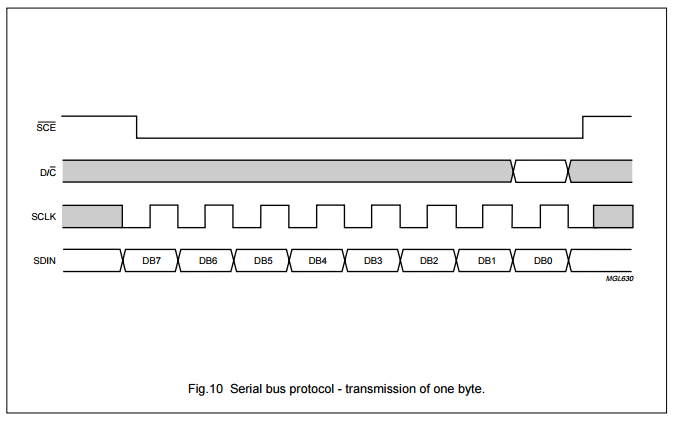
\includegraphics[width=.5\textwidth]{implementation/pcd8544_transmission}
	\caption{Transmission of one byte for the PCD8544\cite[p. 12]{philips:pcd8544}}
	\label{fig:pcd8544_transmission}
\end{figure}

Here in figure\ref{fig:pcd8544_transmission} we see the transmission of one byte.
From this we can see that serialclock enable has to be held low for the duration of the transmission,
and that the data/command has to be set when the last bit is read.


If we do not pull the serialclock enable high again after we are done the display will look for another byte transmission.
We can use this fact to write the entire screen at once, that could be an array reprecentation of the display that we have in ram.


We have implementet functions that does transfer of one byte data or command and a function that can transfer a data array.


\subsubsection{Commands}
The screen has alot of instructions for setup.

\begin{figure}
	\centering
	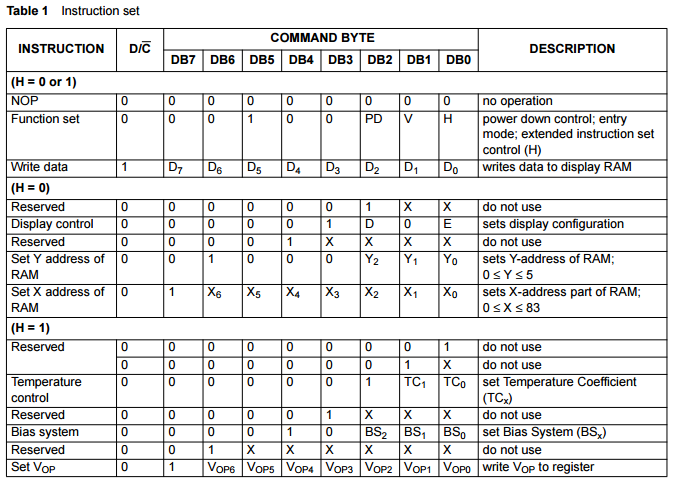
\includegraphics[width=.5\textwidth]{implementation/pcd8544_instructions}
	\caption{Transmission of one byte for the PCD8544\cite[p. 12]{philips:pcd8544}}
	\label{fig:pcd8544_Instructions}
\end{figure}

As seen in figure \ref{ig:pcd8544_Instructions} the display has two instruction sets
one called basic and one called extended, to be able to use all commands you can switch between the two with the function command.

The driver implements all the instructions for the user, but it is up to the user to know whether the display is in extended or basic mode.
This was done to allow for sending more than one instruction and not haveing to change instructionset all the time.
